\chapter{Graph Neural Networks} \label{literature}

\section{Background - Artificial Neural Networks}

\subsection{Introduction}

\subsubsection{Historical Background}

\textbf{Artificial Neural Networks (ANN)}, or sometimes simply called
\textbf{neural networks} is a class of computational models that mimic
the way biological neural networks work, such as the human brain. Interest
on the subject sparked after the seminal paper \textit{"A Logical
Calculus of the Ideas Immanent in Nervous Activity"}
\cite{article:McCulloch1943} by Warren McCulloch and Walter Pitts, where
they proposed a computationally functional model of neural networks.
Their suggestions showed that in principle, any function a digital computer
compute, a neural net should too. The models they described had weights
and thresholds, but they lacked a training method. 

The suggestions of McCulloch and Pitts lead Frank Rosenblatt to create
the \textit{Perceptron} in 1958 \cite{article:Rosenblatt1958ThePa}, a
binary classifier algorithm based on supervised
learning\footnote{Supervised learning is a machine learning training
technique that optimizes a model based on examples input-output
pairs.}. Although initially promising, single layer perceptrons were
not able to train on multiple classes of patterns and were eventually
proven incapable of learning a XOR function \footnote{XOR (Exclusive
or, $x\oplus y$) is a logical operation that is true only if its
arguments differ.} in the book \textit{Perceptrons}
\cite{book:minsky1969perceptrons}, as the way they worked was by
``separating'' data linearly. This lead to a stagnation in machine
learning research dubbed ``AI winter'', until the proposal of
\textbf{backpropagation\footnote{Backpropagation is a method of fine
tuning a neural network based on the error rate obtained from previous
runs of the program. It will be discussed in detail later in this
thesis.}} by Paul John Werbos in 1975 \cite{book:werbos1975beyond}.

A renewed interest in the field lead to the development of the
Cresceptron \cite{article:Cresceptron} in 1992, a method of training
large networks with pooling layers (\textbf{max-pooling}) and down-sampling.
GPU\footnote{GPU - Graphics Processing Units is a specialized
electronic circuit, a central part of modern computers which excels in
efficient computation of algorithms which process large blocks of data
parallelly, thus exceling in machine learning applications.} usage made
possible the training of larger networks, while new types of networks
emerged such as the \textbf{Recurrent Neural Networks (RNNs)}.
\textbf{Convolutional Neural Networks} have recently proven to be
far superior for image classification tasks.

In recent years, neural 


\subsubsection{Summary}

One can think of ANNs as a directed graph, with a collection of nodes
which are densely connected (called \textbf{artificial neurons}),
transimiting signals to each other. These nodes are usually organized
in sets of layers, with signals moving in one direction
(i.e. \textit{feed forward networks}) through weighted connections.
Signals received on a single neuron are real numbers, and the output
of a single neuron is the output of an aggregation of a non-linear
function of the sum of its inputs. This function is called an
\textit{activation function} and its results are propagated to all of
the nodes outgoing connections.  Thus, each neuron can be thought as a
simple processing unit. The weighted connections between nodes might
have an excitatory or inhibitory effect, based on these weights which
can be positive, negative or very close to zero, having no effect
\cite[Chap. ~ 1]{book:Gurney1997AnIT}.  .  While training, training
data is passed through the input layer and gets radically transformed
through the layers until it reaches the output layer. The weights and
other trainable parameters are then adjusted until the training data
consistently reaches satisfactory results.

\begin{figure}[h!]
  \centering
  % % \documentclass[tikz]{standalone}
% \usepackage{tikz}
    \usetikzlibrary{positioning}

\tikzset{basic/.style={draw,fill=blue!50!green!20,text width=1em,text badly centered}}
\tikzset{input/.style={basic,circle}}
\tikzset{weights/.style={basic,rectangle}}
\tikzset{functions/.style={basic,circle,fill=blue!10}}

% \begin{document}
    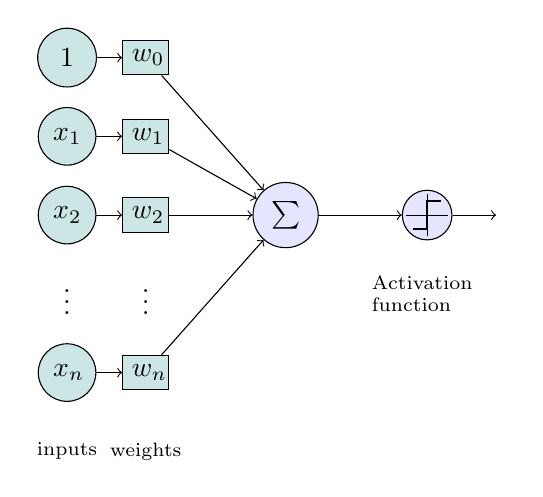
\begin{tikzpicture}
        \node[functions] (center) {};
        \node[below of=center,font=\scriptsize,text width=4em] {Activation function};
        \draw[thick] (0.5em,0.5em) -- (0,0.5em) -- (0,-0.5em) -- (-0.5em,-0.5em);
        \draw (0em,0.75em) -- (0em,-0.75em);
        \draw (0.75em,0em) -- (-0.75em,0em);
        \node[right of=center] (right) {};
            \path[draw,->] (center) -- (right);
        \node[functions,left=3em of center] (left) {$\sum$};
            \path[draw,->] (left) -- (center);
        \node[weights,left=3em of left] (2) {$w_2$} -- (2) node[input,left of=2] (l2) {$x_2$};
            \path[draw,->] (l2) -- (2);
            \path[draw,->] (2) -- (left);
        \node[below of=2] (dots) {$\vdots$} -- (dots) node[left of=dots] (ldots) {$\vdots$};
        \node[weights,below of=dots] (n) {$w_n$} -- (n) node[input,left of=n] (ln) {$x_n$};
            \path[draw,->] (ln) -- (n);
            \path[draw,->] (n) -- (left);
        \node[weights,above of=2] (1) {$w_1$} -- (1) node[input,left of=1] (l1) {$x_1$};
            \path[draw,->] (l1) -- (1);
            \path[draw,->] (1) -- (left);
        \node[weights,above of=1] (0) {$w_0$} -- (0) node[input,left of=0] (l0) {$1$};
            \path[draw,->] (l0) -- (0);
            \path[draw,->] (0) -- (left);
        \node[below of=ln,font=\scriptsize] {inputs};
        \node[below of=n,font=\scriptsize] {weights};
    \end{tikzpicture}
% \end{document}
  \scalebox{.8}{% See https://tikz.net/neural_networks/ for more.
\usetikzlibrary{arrows.meta} % for arrow size
\contourlength{1.4pt}
\tikzset{>=latex} % for LaTeX arrow head
% \usepackage{xcolor}
\colorlet{myred}{red!80!black}
\colorlet{myblue}{blue!80!black}
\colorlet{mygreen}{green!60!black}
\colorlet{myorange}{orange!70!red!60!black}
\colorlet{mydarkred}{red!30!black}
\colorlet{mydarkblue}{blue!40!black}
\colorlet{mydarkgreen}{green!30!black}
\tikzstyle{node}=[thick,circle,draw=myblue,minimum size=22,inner sep=0.5,outer sep=0.6]
\tikzstyle{node in}=[node,green!20!black,draw=mygreen!30!black,fill=mygreen!25]
\tikzstyle{node hidden}=[node,blue!20!black,draw=myblue!30!black,fill=myblue!20]
\tikzstyle{node convol}=[node,orange!20!black,draw=myorange!30!black,fill=myorange!20]
\tikzstyle{node out}=[node,red!20!black,draw=myred!30!black,fill=myred!20]
\tikzstyle{connect}=[thick,mydarkblue] %,line cap=round
\tikzstyle{connect arrow}=[-{Latex[length=4,width=3.5]},thick,mydarkblue,shorten <=0.5,shorten >=1]
\tikzset{ % node styles, numbered for easy mapping with \nstyle
  node 1/.style={node in},
  node 2/.style={node hidden},
  node 3/.style={node out},
}
\def\nstyle{int(\lay<\Nnodlen?min(2,\lay):3)} % map layer number onto 1, 2, or 3
\begin{tikzpicture}[x=2.2cm,y=1.4cm]
  \message{^^JNeural network, shifted}
  \readlist\Nnod{4,5,3} % array of number of nodes per layer
  \readlist\Nstr{n,m,k} % array of string number of nodes per layer
  \readlist\Cstr{\strut x,a^{(\prev)},y} % array of coefficient symbol per layer
  \def\yshift{0.5} % shift last node for dots
  
  \message{^^J  Layer}
  \foreachitem \N \in \Nnod{ % loop over layers
    \def\lay{\Ncnt} % alias of index of current layer
    \pgfmathsetmacro\prev{int(\Ncnt-1)} % number of previous layer
    \message{\lay,}
    \foreach \i [evaluate={\c=int(\i==\N); \y=\N/2-\i-\c*\yshift;
                 \index=(\i<\N?int(\i):"\Nstr[\lay]");
                 \x=\lay; \n=\nstyle;}] in {1,...,\N}{ % loop over nodes
      % NODES
      \node[node \n] (N\lay-\i) at (\x,\y) {$\Cstr[\lay]_{\index}$};
      
      % CONNECTIONS
      \ifnum\lay>1 % connect to previous layer
        \foreach \j in {1,...,\Nnod[\prev]}{ % loop over nodes in previous layer
          \draw[connect,white,line width=1.2] (N\prev-\j) -- (N\lay-\i);
          \draw[connect arrow] (N\prev-\j) -- (N\lay-\i);
          % \draw[connect] (N\prev-\j) -- (N\lay-\i)
          %    node[pos=0.50] {\contour{white}{$w_{1, \index}$}};
          %\draw[connect] (N\prev-\j.0) -- (N\lay-\i.180); % connect to left
        }
      \fi % else: nothing to connect first layer
      
    }
    \path (N\lay-\N) --++ (0,1+\yshift) node[midway,scale=1.5] {$\vdots$};
  }
  
  % LABELS
  \node[above=5,align=center,mygreen!60!black] at (N1-1.90) {input\\[-0.2em]layer};
  \node[above=2,align=center,myblue!60!black] at (N2-1.90) {hidden layer};
  \node[above=10,align=center,myred!60!black] at (N\Nnodlen-1.90) {output\\[-0.2em]layer};
  
\end{tikzpicture}}
  \caption{A simple neural network demonstrating the layered structure and
  and flow of data from input to output.}
  \label{fig:simple_nn_demo}
\end{figure}
\newpage
% \section{Backpropagation}
\section{Mathematics of Artificial Neural Networks}
\subsection{Building Blocks}
% \begin{figure}[t!]
%   \centering
%   % % \documentclass[tikz]{standalone}
% \usepackage{tikz}
    \usetikzlibrary{positioning}

\tikzset{basic/.style={draw,fill=blue!50!green!20,text width=1em,text badly centered}}
\tikzset{input/.style={basic,circle}}
\tikzset{weights/.style={basic,rectangle}}
\tikzset{functions/.style={basic,circle,fill=blue!10}}

% \begin{document}
    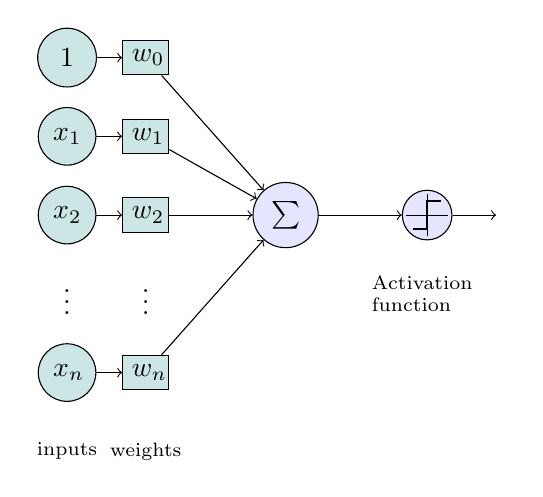
\begin{tikzpicture}
        \node[functions] (center) {};
        \node[below of=center,font=\scriptsize,text width=4em] {Activation function};
        \draw[thick] (0.5em,0.5em) -- (0,0.5em) -- (0,-0.5em) -- (-0.5em,-0.5em);
        \draw (0em,0.75em) -- (0em,-0.75em);
        \draw (0.75em,0em) -- (-0.75em,0em);
        \node[right of=center] (right) {};
            \path[draw,->] (center) -- (right);
        \node[functions,left=3em of center] (left) {$\sum$};
            \path[draw,->] (left) -- (center);
        \node[weights,left=3em of left] (2) {$w_2$} -- (2) node[input,left of=2] (l2) {$x_2$};
            \path[draw,->] (l2) -- (2);
            \path[draw,->] (2) -- (left);
        \node[below of=2] (dots) {$\vdots$} -- (dots) node[left of=dots] (ldots) {$\vdots$};
        \node[weights,below of=dots] (n) {$w_n$} -- (n) node[input,left of=n] (ln) {$x_n$};
            \path[draw,->] (ln) -- (n);
            \path[draw,->] (n) -- (left);
        \node[weights,above of=2] (1) {$w_1$} -- (1) node[input,left of=1] (l1) {$x_1$};
            \path[draw,->] (l1) -- (1);
            \path[draw,->] (1) -- (left);
        \node[weights,above of=1] (0) {$w_0$} -- (0) node[input,left of=0] (l0) {$1$};
            \path[draw,->] (l0) -- (0);
            \path[draw,->] (0) -- (left);
        \node[below of=ln,font=\scriptsize] {inputs};
        \node[below of=n,font=\scriptsize] {weights};
    \end{tikzpicture}
% \end{document}
%   \scalebox{.8}{
\usetikzlibrary{arrows.meta} % for arrow size
\contourlength{1.4pt}
\tikzset{>=latex} % for LaTeX arrow head
\colorlet{myred}{red!80!black}
\colorlet{myblue}{blue!80!black}
\colorlet{mygreen}{green!60!black}
\colorlet{myorange}{orange!70!red!60!black}
\colorlet{mydarkred}{red!30!black}
\colorlet{mydarkblue}{blue!40!black}
\colorlet{mydarkgreen}{green!30!black}
\tikzstyle{node}=[thick,circle,draw=myblue,minimum size=22,inner sep=0.5,outer sep=0.6]
\tikzstyle{node in}=[node,green!20!black,draw=mygreen!30!black,fill=mygreen!25]
\tikzstyle{node hidden}=[node,blue!20!black,draw=myblue!30!black,fill=myblue!20]
\tikzstyle{node convol}=[node,orange!20!black,draw=myorange!30!black,fill=myorange!20]
\tikzstyle{node out}=[node,red!20!black,draw=myred!30!black,fill=myred!20]
\tikzstyle{connect}=[thick,mydarkblue] %,line cap=round
\tikzstyle{connect arrow}=[-{Latex[length=4,width=3.5]},thick,mydarkblue,shorten <=0.5,shorten >=1]
\tikzset{ % node styles, numbered for easy mapping with \nstyle
  node 1/.style={node in},
  node 2/.style={node hidden},
  node 3/.style={node out},
}
\def\nstyle{int(\lay<\Nnodlen?min(2,\lay):3)} % map layer number onto 1, 2, or 3



\begin{tikzpicture}[x=2.2cm,y=1.4cm]
  \message{^^JNeural network, shifted}
  \readlist\Nnod{4,5,3}
  \readlist\Nstr{n,m,k}
  \readlist\Cstr{\{\strut x, a^{(\prev)},y}
  \def\yshift{0.5}

  \message{^^J Layer}
  \foreachitem \N \in \Nnod{
    \def\lay{\Ncnt} % alias of index of current layer
    \pgfmathsetmacro\prev{int(\Ncnt-1)} % number of previous layer
    \message{\lay,}
    \foreach \i [evaluate={\c=int(\i==\N); \y=\N/2-\i-\c*\yshift;
                 \index=(\i<\N?int(\i):"\Nstr[\lay]");
                 \x=\lay; \n=\nstyle;}] in {1,...,\N}{
                 \node[node hidden] (N\lay-\i) at (\x,\y) {$\Cstr[\lay]_{\index}$};
        \ifnum\lay>1 % connect to previous layer
                 % \node[node hidden] (N\lay-\i) at (\x,\y) {$\Cstr[\lay]_{\index}$};
            \foreach \j in {1,...,\Nnod[\prev]}{ % loop over nodes in previous layer
            \draw[connect,white,line width=1.2] (N\prev-\j) -- (N\lay-\i);
            \draw[connect arrow] (N\prev-\j) -- (N\lay-\i);
            \draw[connect] (N\prev-\j) -- (N\lay-\i)
            node[pos=0.50] {\contour{white}{$w_{1, \index}$}};
            }
          % \else
          %   \node[node,blue!20!black!80,draw=myblue!20,fill=myblue!5]
          %   \node[node hidden] (N\lay-\i) at (\x,\y) {$\Cstr[\lay]_{\index}$};
          %   \foreach \j in {1,...,\Nnod[\prev]}{ % loop over nodes in previous layer
          %   \draw[connect,white,line width=1.2] (N\prev-\j) -- (N\lay-\i);
          %   \draw[connect arrow] (N\prev-\j) -- (N\lay-\i);
          % }
          \fi
          }

            
    \path (N\lay-\N) --++ (0,1+\yshift) node[midway,scale=1.5] {$\vdots$};



                 
               } % loop over nodes
  
\end{tickzpicture}



% \begin{tikzpicture}[x=2.7cm,y=1.6cm]
%   \message{^^JNeural network activation}
%   \def\NI{5} % number of nodes in input layers
%   \def\NO{4} % number of nodes in output layers
%   \def\yshift{0.4} % shift last node for dots
  
%   % INPUT LAYER
%   \foreach \i [evaluate={\c=int(\i==\NI); \y=\NI/2-\i-\c*\yshift; \index=(\i<\NI?int(\i):"n");}]
%               in {1,...,\NI}{ % loop over nodes
%     \node[node in,outer sep=0.6] (NI-\i) at (0,\y) {$a_{\index}^{(0)}$};
%   }
  
%   % OUTPUT LAYER
%   \foreach \i [evaluate={\c=int(\i==\NO); \y=\NO/2-\i-\c*\yshift; \index=(\i<\NO?int(\i):"m");}]
%     in {\NO,...,1}{ % loop over nodes
%     \ifnum\i=1 % high-lighted node
%       \node[node hidden]
%         (NO-\i) at (1,\y) {$a_{\index}^{(1)}$};
%       \foreach \j [evaluate={\index=(\j<\NI?int(\j):"n");}] in {1,...,\NI}{ % loop over nodes in previous layer
%         \draw[connect,white,line width=1.2] (NI-\j) -- (NO-\i);
%         \draw[connect] (NI-\j) -- (NO-\i)
%           node[pos=0.50] {\contour{white}{$w_{1,\index}$}};
%       }
%     \else % other light-colored nodes
%       \node[node,blue!20!black!80,draw=myblue!20,fill=myblue!5]
%         (NO-\i) at (1,\y) {$a_{\index}^{(1)}$};
%       \foreach \j in {1,...,\NI}{ % loop over nodes in previous layer
%         %\draw[connect,white,line width=1.2] (NI-\j) -- (NO-\i);
%         \draw[connect,myblue!20] (NI-\j) -- (NO-\i);
%       }
%     \fi
%   }
  
%   % DOTS
%   \path (NI-\NI) --++ (0,1+\yshift) node[midway,scale=1.2] {$\vdots$};
%   \path (NO-\NO) --++ (0,1+\yshift) node[midway,scale=1.2] {$\vdots$};

%  \end{tikzpicture}
          % ifnum \i=1
          % \draw[connect] (N\prev-\j) -- (N\lay-\i)
          %    node[pos=0.50] {\contour{white}{$w_{1, \index}$}};
          %    \fi}
%   \caption{A simple neural network demonstrating the layered structure and
%   and flow of data from input to output.}
%   \label{fig:nn_activation}
% \end{figure}

As mentioned before, the building blocks of ANNs are its artificial
neurons organized into layers. In  \fref{fig:simple_nn_demo} a basic
ANN is presented, demonstrating the different layers that are typically
present in a feedforward neural network \footnote{Feedforward Neural Networks
  (FNNs) are the simplest type of neural networks, with the information moving
  only in one direction (``forward'' through the layers), without any loops or
  cycles \cite{article:SCHMID}. Different types of neural networks are discussed
  later.} while the building blocks are widely considered \cite{article:SCHMID} to
be:
\begin{itemize}
\item \textbf{Input layer} This layer's purpose is to act as an
  entrypoint to the neural network and performs no computations. Data moves from
  this layer to the hidden layer succeeding it.
\item \textbf{Hidden layer} Networks typically have one or more
  hidden layers, in which some computation takes place. Data moves from the input
  layer to a hidden layer where it is transformed and together with its weights
  moves to the next hidden layer or the output layer.
\item \textbf{Output layer} Transformed data ``exits'' the network here,
  where it can pass through some function to reach the desired output
  format
\item \textbf{Edges and Weights} Each node in a layer is connected
  to a set (usually all) of the nodes of the following layer with a
  weighted edge. Signals from node $i$ of layer $k$ will be the input
  of node $j$ of layer $l$, multiplied by a weight $W_{ij}$. 
\item \textbf{Activation Functions} An activation function takes as
  input some form of aggregate (usually the weighted sum) of the signals
  arriving at a node and produces an output. This function is typically
  nonlinear and differentiable for reasons which will be discussed later.
\item \textbf{Learning} The learning process in a ANN involves modifying
  its weights and other learnable parameters to improve the accuracy
  of the result on the output layer. Learning usually involves a cost
  function which is evaluated on a predefined basis and adjustments are
  made accordingly. One of the most widespread learning techniques is
  \textit{backpropagation}, where the error is propagated backwards
  through the network.
  
\end{itemize}
Along with the data from previous layers aggregated at a neuron, a bias
is typically added which acts in the same way the intercept does in a
linear equation. It adjusts the output of the activation function along
with the weighted sum of the inputs to the neuron. It is also a trainable
constant value provided to each node of a layer. Biases are node level
parameters and do not depend on values provided by previous layers.

All of the computations that take place in layer can be represented in
a compact matrix form, as shown below.

\begin{figure}[h!]
  \centering
  % % \documentclass[tikz]{standalone}
% \usepackage{tikz}
    \usetikzlibrary{positioning}

\tikzset{basic/.style={draw,fill=blue!50!green!20,text width=1em,text badly centered}}
\tikzset{input/.style={basic,circle}}
\tikzset{weights/.style={basic,rectangle}}
\tikzset{functions/.style={basic,circle,fill=blue!10}}

% \begin{document}
    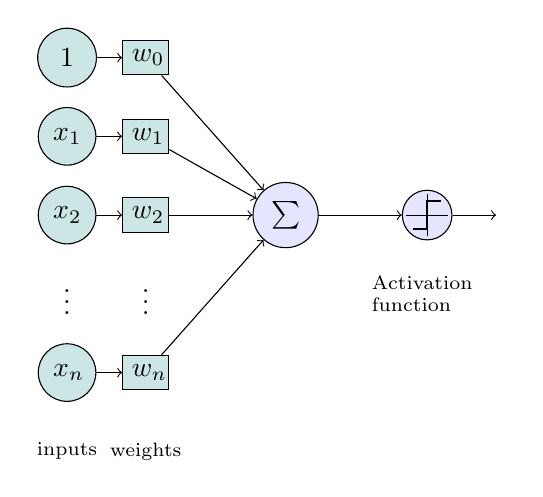
\begin{tikzpicture}
        \node[functions] (center) {};
        \node[below of=center,font=\scriptsize,text width=4em] {Activation function};
        \draw[thick] (0.5em,0.5em) -- (0,0.5em) -- (0,-0.5em) -- (-0.5em,-0.5em);
        \draw (0em,0.75em) -- (0em,-0.75em);
        \draw (0.75em,0em) -- (-0.75em,0em);
        \node[right of=center] (right) {};
            \path[draw,->] (center) -- (right);
        \node[functions,left=3em of center] (left) {$\sum$};
            \path[draw,->] (left) -- (center);
        \node[weights,left=3em of left] (2) {$w_2$} -- (2) node[input,left of=2] (l2) {$x_2$};
            \path[draw,->] (l2) -- (2);
            \path[draw,->] (2) -- (left);
        \node[below of=2] (dots) {$\vdots$} -- (dots) node[left of=dots] (ldots) {$\vdots$};
        \node[weights,below of=dots] (n) {$w_n$} -- (n) node[input,left of=n] (ln) {$x_n$};
            \path[draw,->] (ln) -- (n);
            \path[draw,->] (n) -- (left);
        \node[weights,above of=2] (1) {$w_1$} -- (1) node[input,left of=1] (l1) {$x_1$};
            \path[draw,->] (l1) -- (1);
            \path[draw,->] (1) -- (left);
        \node[weights,above of=1] (0) {$w_0$} -- (0) node[input,left of=0] (l0) {$1$};
            \path[draw,->] (l0) -- (0);
            \path[draw,->] (0) -- (left);
        \node[below of=ln,font=\scriptsize] {inputs};
        \node[below of=n,font=\scriptsize] {weights};
    \end{tikzpicture}
% \end{document}
  \scalebox{1}{
\tikzset{>=latex} % for LaTeX arrow head
\colorlet{myred}{red!80!black}
\colorlet{myblue}{blue!80!black}
\colorlet{mygreen}{green!60!black}
\colorlet{myorange}{orange!70!red!60!black}
\colorlet{mydarkred}{red!30!black}
\colorlet{mydarkblue}{blue!40!black}
\colorlet{mydarkgreen}{green!30!black}
\tikzstyle{node}=[thick,circle,draw=myblue,minimum size=22,inner sep=0.5,outer sep=0.6]
\tikzstyle{node in}=[node,green!20!black,draw=mygreen!30!black,fill=mygreen!25]
\tikzstyle{node hidden}=[node,blue!20!black,draw=myblue!30!black,fill=myblue!20]
\tikzstyle{node convol}=[node,orange!20!black,draw=myorange!30!black,fill=myorange!20]
\tikzstyle{node out}=[node,red!20!black,draw=myred!30!black,fill=myred!20]
\tikzstyle{connect}=[thick,mydarkblue] %,line cap=round
\tikzstyle{connect arrow}=[-{Latex[length=4,width=3.5]},thick,mydarkblue,shorten <=0.5,shorten >=1]
\tikzset{ % node styles, numbered for easy mapping with \nstyle
  node 1/.style={node in},
  node 2/.style={node hidden},
  node 3/.style={node out},
}
\def\nstyle{int(\lay<\Nnodlen?min(2,\lay):3)} % map layer number onto 1, 2, or 3



\begin{tikzpicture}[x=2.7cm,y=1.6cm]
  \message{^^JNeural network activation}
  \def\NI{5} % number of nodes in input layers
  \def\NO{4} % number of nodes in output layers
  \def\yshift{0.4} % shift last node for dots
  
  % INPUT LAYER
  \foreach \i [evaluate={\c=int(\i==\NI); \y=\NI/2-\i-\c*\yshift; \index=(\i<\NI?int(\i):"n");}]
              in {1,...,\NI}{ % loop over nodes
    \node[node in,outer sep=0.6] (NI-\i) at (0,\y) {$a_{\index}^{(0)}$};
  }
  
  % OUTPUT LAYER
  \foreach \i [evaluate={\c=int(\i==\NO); \y=\NO/2-\i-\c*\yshift; \index=(\i<\NO?int(\i):"m");}]
    in {\NO,...,1}{ % loop over nodes
    \ifnum\i=1 % high-lighted node
      \node[node hidden]
        (NO-\i) at (1,\y) {$a_{\index}^{(1)}$};
      \foreach \j [evaluate={\index=(\j<\NI?int(\j):"n");}] in {1,...,\NI}{ % loop over nodes in previous layer
        \draw[connect,white,line width=1.2] (NI-\j) -- (NO-\i);
        \draw[connect] (NI-\j) -- (NO-\i)
          node[pos=0.50] {\contour{white}{$w_{1,\index}$}};
      }
    \else % other light-colored nodes
      \node[node,blue!20!black!80,draw=myblue!20,fill=myblue!5]
        (NO-\i) at (1,\y) {$a_{\index}^{(1)}$};
      \foreach \j in {1,...,\NI}{ % loop over nodes in previous layer
        %\draw[connect,white,line width=1.2] (NI-\j) -- (NO-\i);
        \draw[connect,myblue!20] (NI-\j) -- (NO-\i);
      }
    \fi
  }
  
  % DOTS
  \path (NI-\NI) --++ (0,1+\yshift) node[midway,scale=1.2] {$\vdots$};
  \path (NO-\NO) --++ (0,1+\yshift) node[midway,scale=1.2] {$\vdots$};
  
  % EQUATIONS
  \def\agr#1{{\color{mydarkgreen}a_{#1}^{(0)}}}
  \node[below=17,right=11,mydarkblue,scale=0.95] at (NO-1)
    {$\begin{aligned} %\underset{\text{bias}}{b_1}
       &= \color{mydarkred}\sigma\left( \color{black}
            w_{1,1}\agr{1} + w_{1,2}\agr{2} + \ldots + w_{1,n}\agr{n} + b_1^{(0)}
          \color{mydarkred}\right)\\
       &= \color{mydarkred}\sigma\left( \color{black}
            \sum_{i=1}^{n} w_{1,i}\agr{i} + b_1^{(0)}
           \color{mydarkred}\right)
     \end{aligned}$};
  \node[right,scale=0.9] at (1.3,-1.3)
    {$\begin{aligned}
      {\color{mydarkblue}
      \begin{pmatrix}
        a_{1}^{(1)} \\[0.3em]
        a_{2}^{(1)} \\
        \vdots \\
        a_{m}^{(1)}
      \end{pmatrix}}
      &=
      \color{mydarkred}\sigma\left[ \color{black}
      \begin{pmatrix}
        w_{1,1} & w_{1,2} & \ldots & w_{1,n} \\
        w_{2,1} & w_{2,2} & \ldots & w_{2,n} \\
        \vdots  & \vdots  & \ddots & \vdots  \\
        w_{m,1} & w_{m,2} & \ldots & w_{m,n}
      \end{pmatrix}
      {\color{mydarkgreen}
      \begin{pmatrix}
        a_{1}^{(0)} \\[0.3em]
        a_{2}^{(0)} \\
        \vdots \\
        a_{n}^{(0)}
      \end{pmatrix}}
      +
      \begin{pmatrix}
        b_{1}^{(0)} \\[0.3em]
        b_{2}^{(0)} \\
        \vdots \\
        b_{m}^{(0)}
      \end{pmatrix}
      \color{mydarkred}\right]\\[0.5em]
      {\color{mydarkblue}a^{(1)}}
      &= \color{mydarkred}\sigma\left( \color{black}
           \mathbf{W}^{(0)} {\color{mydarkgreen}a^{(0)}}+\mathbf{b}^{(0)}
         \color{mydarkred}\right)
         %\color{black},\quad \mathbf{W}^{(0)} \in \mathbb{R}^{m\times n}
    \end{aligned}$};
  
\end{tikzpicture}
}
  \caption{Input to a single neuron in a feedforward network. Here $\sigma$ represents
    the activation function and the exponents represent layers. The activation of a layer
    can be conveniently represented in matrix form. Biases are added to the input of the
    node.}
  \label{fig:nn_activation}
\end{figure}

% TODO: Describe deep learning (multiple layers?)

\subsection{Types of the most common ANNs}

\subsubsection{Feedforward Networks}

\textbf{Feedforward neural networks (FNNs)} are the exemplary of ANNs, and the first to be
conceived and created by Rosenblatt in 1958 with the creation of the
perceptron \cite{article:Rosenblatt1958ThePA}. Their goal is to approximate
some function $f^{*}$; i.e. a classifier uses the function
$y=f^{*}(\bm{x})$ to map the input $\bm{x}$ to some category $y$. The
goal of a feedforward network would then be to define a mapping
$\bm{y} = f(\bm{x};~\bm{\theta})$ and train in a way that the values
of the parameter vector $\bm{\theta}$ provide the best approximation of
the function $f^{*}$.

These networks are called feedforward as information flows from the input layer
$\bm{x}$ through intermediate computational layers used to define $\bm{f}$ and
finally to the output $\bm{y}$. There are no loops providing (called
\textbf{feedback connections}) information from the output back into
the input or other intermediate layers of the network.

Feedforward networks can be thought as a chain of functions, composing
the final structure of the network. As an example, consider a network
with three of these functions as $f(\bm{x}) = f^{(3)}(f^{(2)}(f^{(1)}(\bm{x})))$.
In this case, the exponents denotes the layer, with $f^{(1)}$ beign the first
layer, $f^{(2)}$ the second etc. The total number of these functions is called
the \textbf{depth} of the NN and the terminology ``deep learning'' arose from
this layered structure.

During training the goal is to modify the parameters of the
network in a way that $f(\bm{x})$ closely matches $f^*(\bm{x})$. The training
set is composed of pairs of $\bm{x}$ and labels $y \approx f^*(\bm{x})$ and
the output of the network is evaluated at different training points. Training
data defines the exact result expected from each input $\bm{x}$, a value as close
as possible to $y$. The rest of the layers can have arbitary behaviours as long
as they transform the data in a way defined by the training goal. The
learning algorithm can ``use'' them in any way that is useful to it, and
the training data has no immediate effect on their behaviour. They are
thus called \textbf{``hidden layers''} as they do not produce any
useful output. 

\subsubsection*{Common FNNs}
% In feedforward neural networks, information flows from the input
% \textbf{$x$} layer towards the output


\subsection{Training}



\newpage
\subsection{Convolutional Neural Networks}
\newpage

